\documentclass[10pt,a4paper]{article}
\usepackage[utf8]{inputenc}  
\usepackage[T1]{fontenc}       
\usepackage[francais]{babel}
\usepackage{fullpage}
%\usepackage{euler}
\usepackage{amsmath}
%\usepackage{framed}
\usepackage{amsfonts}
\usepackage{amssymb}
\usepackage{pifont}
\usepackage{mathrsfs}
\usepackage{graphicx}
\usepackage{wasysym}
\usepackage{pstricks-add}
\usepackage[squaren,Gray]{SIunits}
\usepackage[a4paper]{geometry}
\geometry{hscale=0.86,vscale=0.87,centering}



\pagestyle{empty}

%\newcommand{\Titre}[4]{\noindent \textsc{#1}} \hfill \textbf{\textsc{#2}}\\ #3 \hfill \emph{#4}\\  \hrule\vspace{\baselineskip}}

\newcommand{\Titre}[3]{\begin{center} {\LARGE\textbf{\textsc{#1}}}\\ #2 \hfill \emph{#3} \\  \hrule\vspace{\baselineskip}\end{center}}

\begin{document}

\Titre{Correction du DM de Physique}{Asp J.Buet}{17 décembre 2013}
\thispagestyle{plain}
\pagestyle{plain}


\part*{L'appareil photographique}

\bigskip
\section{Optique d'un appareil photo}

\begin{enumerate}
\item Il faut que les rayons soient proches de l'axe optique et peu inclinés par rapport à l'axe optique.
\item La distance de l'objectif au plan de la pellicule est égale à la distance focale de l'objectif $f'_{obj}$.
\smallskip
\item \textbf{Pouvoir de résolution}

\begin{figure}[h!]
\center
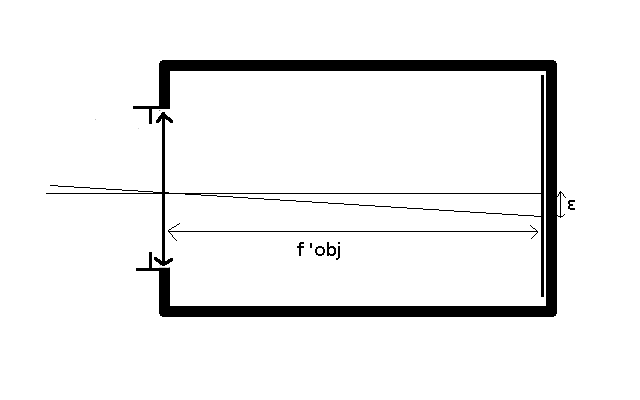
\includegraphics[scale=0.45]{pouvoir_resolution.png}
\end{figure}

On note $\alpha$ l'angle minimum entre deux objets à l'infini pour qu'ils soient perçus séparément par l'appareil photo. Il faut donc que les rayons provenant
de l'un et ceux provenant de l'autre arrivent dans deux récepteurs différents. L'appareil photo étant réglé pour une mise au point à l'infini, on a donc, 
d'après le schéma (on dessine les rayons passant par le centre optique) un angle minimum $\boxed{\tan\alpha=\alpha=\frac{\varepsilon}{f'_{obj}}}$
\smallskip
\item \textbf{Profondeur de champ}

Pour une distance $L$ fixée entre l'objectif et la pellicule, un objet qui est parfaitement net se situe à une distance $\overline{OA}$ donnée par la relation
de conjugaison : $$\frac{1}{L}-\frac{1}{\overline{OA}}=\frac{1}{f'_{obj}}$$
On a donc $\boxed{\overline{OA}=\frac{L.f'_{obj}}{f'_{obj}-L}}$.

Un point à la limite de la netteté fait une tache sur l'écran de largeur $\varepsilon$. Comme le montrent les schémas ci-dessous, il y a deux tels points.
\begin{figure}[h!]
\begin{minipage}{0.4\textwidth}
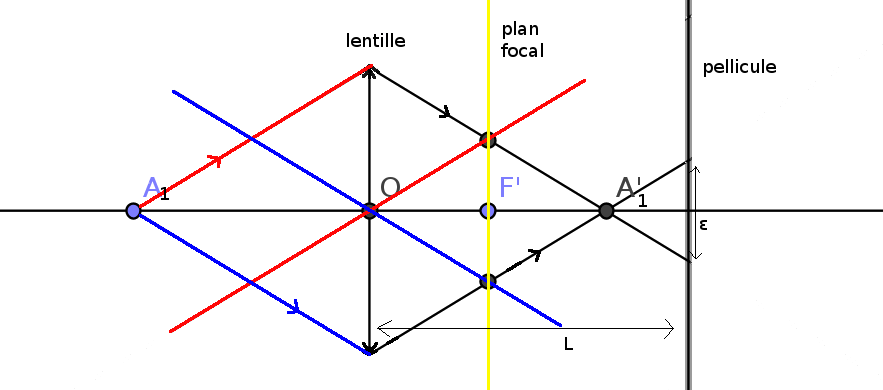
\includegraphics[scale=1.3]{profondeur_champ.png}
\end{minipage}
\hfill
\begin{minipage}{0.4\textwidth}
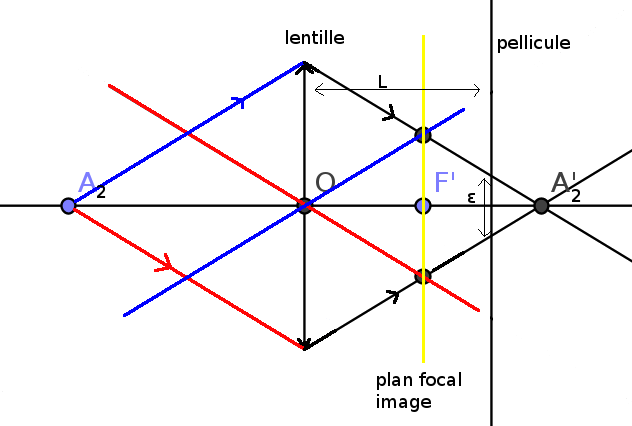
\includegraphics[scale=1.3]{profondeur_champ_2.png}
\end{minipage}
\end{figure}

En limite de netteté on a donc dans le premier cas, en appliquant le théorème de Thalès dans le triangle formé par $OA'_1$ et le côté d'une demi-lentille : 
$\frac{\varepsilon}{D}=\frac{L-\overline{OA'_1}}{\overline{OA'_1}}$, ce qui nous donne $\overline{OA'_1}=\frac{D.L}{D+\varepsilon}$. On en déduit ensuite avec
les formules de conjugaison que $\overline{OA_1}=\frac{\overline{OA'_1}.f'_{obj}}{f'_{obj}-\overline{OA'_1}}$ soit 
$\overline{OA_1}=\frac{D.L.f'_{obj}}{f'_{obj}.(D+\varepsilon)-D.L}$.
\smallskip

Dans le second cas, avec la même méthode on a $\frac{\varepsilon}{D}=\frac{\overline{OA'_2}-L}{\overline{OA'_2}}$, soit 
$\overline{OA'_2}=\frac{D.L}{D-\varepsilon}$ La formule de conjugaison ne change pas et on a donc pour la deuxième position
on a donc $\overline{OA_2}=\frac{D.L.f'_{obj}}{f'_{obj}.(D-\varepsilon)-D.L}$.
\smallskip

Donc l'écart entre ces deux points $A_1$ et $A_2$ donne la profondeur de champ. 

$\overline{A_1A_2}=\overline{A_1O}+\overline{OA_2}=\overline{OA_2}-\overline{OA_1}=
D.L.f'_{obj}.(\frac{1}{f'_{obj}(D-\varepsilon)-D.L}-\frac{1}{f'_{obj}(D+\varepsilon)-D.L})$

Finalement l'expression de la profondeur de champ est :
 $$\boxed{D.L.f'_{obj}.\frac{2.\varepsilon.f'_{obj}}{(f'_{obj}(D-\varepsilon)-D.L).(f'_{obj}(D+\varepsilon)-D.L)}}$$

\item La distance minimale théorique est $\unit{50}{\milli\meter}$, si on approche davantage l'objet, l'image par la lentille est virtuelle et ne peut donc
pas se former sur la pellicule.

Il s'agit, pour la deuxième partie de la question, de trouver la distance à laquelle se situe un objet dont l'image est nette sur la pellicule, située à une
distance $L=\unit{55}{\milli\meter}$ de l'objectif (donc de la lentille).
La relation de conjugaison nous donne donc : $\overline{OA}=\frac{\overline{OA'}.f'_{obj}}{f'_{obj}-\overline{OA'}}$. Or $\overline{OA'}=L$ donc 
$\boxed{\overline{OA}=\frac{L.f'_{obj}}{f'_{obj}-L}}$. L'application numérique donne $\underline{\overline{OA}=-\unit{55}{\centi\meter}}$
\item Pour que l'image reste nette, il faut que la tache centrale de diffraction soit contenue à l'intérieur d'un photorécepteur. Il faut donc avoir
$\alpha.f'_{obj}\leqslant \varepsilon/2$, soit $\boxed{N\leqslant \frac{\varepsilon}{2,44.\lambda}}$.

L'application numérique donne $\underline{N\leqslant 20,5}$.
\end{enumerate}
\section{Développement des photographies}
\begin{enumerate}
\item On commence par calculer la quantité de matière pour chacun des solides ioniques. On a donc $M_{K_2CO_3}=2.M_K+M_C+3.M_O=\unit{138}{\gram\per\mole}$ et
$M_{KBr}=M_K+M_{Br}= \unit{119}{\gram\per\mole}$. Ce qui nous donne donc les quantités de matière suivantes : $n_{K_2CO_3}=\unit{0,25}{\mole}$ et 
$n_{KBr}=\unit{2,0.10^{-2}}{\mole}$

On écrit ensuite l'équation de dissolution du solide ionique dans l'eau. On suppose que celui-ci se dissout totalement. On a donc la quantité de matière de
$CO_3^{2-}$ et de $Br^-$ présents en solution. Puisqu'il est donné dans l'énoncé que le volume est $\unit{500}{\milli\liter}$, on a finalement une concentration
$\underline{[CO_3^{2-}]=\unit{0,500}{\mole\per\liter}}$ et $\underline{[Br^-]=\unit{4,0.10^{-2}}{\mole\per\liter}}$.
\item 
\begin{enumerate}
\item $CO_3^{2-}+H_2O\rightleftharpoons HO^-+HCO_3^-$
\item On a $K_a=\frac{[H_3O^+].[CO_3^{2-}]}{[HCO_3^-]}$ d'une part. 

D'autre part, en utilisant l'équation de la réaction écrite à la question précédente, on trouve que $[HCO_3^-]=[OH^-]=\frac{K_e}{[H_3O^+]}$.

En utilisant la conservation de la quantité de matière, puisque la réaction se passe à volume constant, on a aussi : $[HCO_3^-]+[CO_3^{2-}]=[CO_3^{2-}]_0$.
Or $CO_3^{2-}$ est une base faible, on a donc $[HCO_3^-]\ll [CO_3^{2-}]$, ce qui revient à dire que $[CO_3^{2-}]\simeq [CO_3^{2-}]_0$.

Finalement on a donc $K_a=\frac{[H_3O^+]^2.[CO_3^{2-}]_0}{K_e}$, en passant au log on obtient $\boxed{pH=\frac{1}{2}(pK_a+pK_e+log[CO_3^{2-}]_0)}$.
L'application numérique donne $\underline{pH=11,9}$.
\item Le diagramme de prédominance est le suivant :
\begin{figure}[h!]
\center
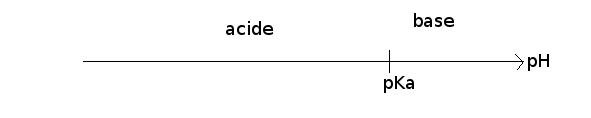
\includegraphics[scale=2]{echelle_pH.png}
\end{figure}

Or $CO_3^{2-}$ est majoritaire, donc le pH est entre 10,2 et 14, soit environ autour de 12.
\end{enumerate}
\item
\begin{enumerate}
\item $$Ag^+_{(aq)} + e^- = Ag_{(s)}$$
$${C_6H_4O_2}_{(aq)}+2H^+_{(aq)}+2e^-={C_6H_6O_2}_{(aq)}$$
\item $$\boxed{2Ag^+_{(aq)}+{C_6H_6O_2}_{(aq)}\longrightarrow 2Ag_{(s)}+2H^+_{(aq)}+{C_6H_4O_2}_{(aq)}}$$
\end{enumerate}
\item 
\begin{enumerate}
\item $K_s=[Ag^+][Br^-]$, lorsque l'on dissout du $AgBr$ dans de l'eau pur, on obtient la même concentration en $Ag^+$ et en $Br^-$. On a donc $K_s=s^2$, soit
$\boxed{s=\sqrt{K_s}}$. L'application numérique donne $s=\unit{5,62.10^{-7}}{\mole\per\liter}$
\item
\begin{enumerate}
\item Le révélateur contient déjà des ions bromures qui sont pris en compte lors du calcul de $K_s$. Puisque $K_s$ est constant et que $[Br^-]$ augmente,
$[Ag^+]$ diminue.
\item On a toujours $K_s=[Ag^+][Br^-]$ mais désormais, s'il y a une concentration $c$ en $Ag^+$, il y a une concentration $[Br^-]_0+c$ en $Br^-$, où
 $[Br^-]_0$ correspond à la concentration déjà présente en solution et calculée au début de l'exercice.

On a donc $K_s=s'.(s'+[Br^-]_0)$. On peut résoudre l'équation du second degré, mais $s'$ va être très petit (on peut voir grâce à la question précédente que
$s$ est déjà petit devant la valeur de $[Br^-]_0$ et $s'$ va être encore plus petit). On résout donc $\boxed{K_s=s'[Br^-]_0}$ (car si $s'$ est petit, $s'^2$ 
est vraiment très petit). On trouve donc $\underline{s'=\unit{7,9.10^{-12}}{\mole\per\liter}}$.
\item L'effet de voile vient du fait qu'il y a des ions argents de la pellicule qui se dissolvent dans la solution et réagissent avec le réducteur pour
former des  atomes d'argent solide uniformément sur toute la pellicule et qui viennent donc former
une traînée blanche sur la photo (sur le négatif, il n'y a plus de zones vraiment blanches, toutes sont devenues un peu foncées, donc l'image finale
est comme derrière un voile blanc). On appelle le bromure de potassium anti-voile parce qu'il vient limiter grandement cette dissolution des cristaux d'argent
contenus dans la pellicule. En effet, sans bromure de potassium on a $[Ag^+]=\unit{5,62.10^{-7}}{\mole\per\liter}$ alors qu'avec le bromure de potassium on a
$[Ag^+]=\unit{7,9.10^{-12}}{\mole\per\liter}$.
\end{enumerate}
\end{enumerate}
\end{enumerate}

\end{document}
